\section{The Eight Point Algorithm}

\paragraph{Introduction} We implement the eight-point algorithm to estimate the fundamental matrix $F$ given two images representing two views of the same scene, which allows us to relate points in one image to epipolar lines in the other. Given eight points correspondences, we derive a linear system where the unknown are the entries of the fundamental matrix by transforming the epipolar constraints using the \textit{Kronecker product trick}. We normalize the points using \textit{Hartley normalization} and we approximate a solution to the linear system using SVD. The entire process is repeated multiple times according to the \textit{RANSAC} framework for robust estimation.

\paragraph{Notation} In this section, we use the following notation:

\begin{itemize}
    \item $\mathbf{x}_i$, $\mathbf{x}'_i$: corresponding points in the first and second image in homogeneous coordinates.
    \item $F$: the fundamental matrix, to be estimated.
    \item $l_i$, $l'_i$: epipolar lines in the first and second image corresponding to $\mathbf{x}'_i$ and $\mathbf{x}_i$.
\end{itemize}

\paragraph{Background}

The fundamental matrix $F$ is the unique $3 \times 3$ rank-2 homogeneous matrix that satisfies the epipolar constraint for any pair of corresponding points $\mathbf{x}_i$ and $\mathbf{x}'_i$:
\begin{align*}
    {\mathbf{x}'_i}^T F \mathbf{x}_i = 0 \quad \text{s.t. } Rank(F)=2
\end{align*}
For a point $\mathbf{x}_i$ ($ \mathbf{x}'_i$) in the first (second) image, the corresponding epipolar line $l'_i$ ($l_i$) in the second (first) image can be computed as:
\begin{align*}
l'_i = F \mathbf{x}_i \quad (l_i = F^T \mathbf{x}'_i)
\end{align*}
Given a point $\mathbf{x}_i$ and its corresponding point $\mathbf{x}_i'$, we defune the \textit{geometric error} $E(\mathbf{x}_i)$ as:
\begin{align*}
    E(\mathbf{x}) = \operatorname{distance}(\mathbf{x}_i, F^T \mathbf{x}'_i)
\end{align*}
Where $\operatorname{distance}(\cdot,\cdot)$ measures the euclidean distance.

\paragraph{Methodology} Our implementation is broken down in the following steps:

\begin{enumerate}
    \item We obtain $30$ point correspondences $\{(\mathbf{x}_i, \mathbf{x}'_i)\}_{i=1}^{30}$ between two images using manual annotation\footnote{We developed another ad-hoc annotator file to obtain pixel-precise manual point correspondences. We also attempted to use \textit{SIFT} for automatic feature detection and matching, but it did not produce satisfactory results in our experiments, so we stick with manual annotation.}.
    
    \item We use \textit{Hartley normalization} to improve numerical stability by transforming the points such that their mean is zero and the average distance from the origin is $\sqrt{2}$. We compute and store the matrices $T_1, T_2$ performing this linear transformation on the two set of points (to later transform the fundamental matrix back):
    \begin{align*}
        \tilde{\mathbf{x}}_i &= T_1\mathbf{x}_i \\
        \tilde{\mathbf{x}}_i &= T_2\mathbf{x}_i
    \end{align*}

\item We use the \textit{Eight points algorithm} to estimate the fundamental matrix $F$:
\begin{enumerate}
    \item Randomly sample a subset of $8$ correspondences
    \item Exploit the \textit{Kronecker product trick} and the epipolar constraints to set up a system of $8$ linear equations in $9$ unknowns (the entries of the matrix $F$).
    \begin{align*}
        x'_i x_i f_{11} + x'_i y_i f_{12} + x'_i f_{13} + y'_i x_i f_{21} + y'_i y_i f_{22} + y'_i f_{23} + x_i f_{31} + y_i f_{32} + f_{33} = 0 \quad \text{for } i=1,...,8
    \end{align*}
    Where $\tilde{\mathbf{x}}_i = (x_i, y_i, 1), \tilde{\mathbf{x}}'_i = (x'_i,y'_i, 1)$ and $f_{ii}$ are the entries of the matrix $F$.
    \item Solve the system via SVD and reshape the solution into a $3 \times 3$ matrix.
    \item Use SVD again to get the best rank-2 approximation of this matrix by setting the last singular value to $0$. Call this reconstructed matrix $\tilde{F}$.
    \item De-normalize $F$ such that it operates on points that are not Hartley normalized:
    \begin{align*}
        F = T_2^\top \tilde{F} T_1
    \end{align*}
    \item Scale it such that $F_{2,2} = 1$ (common convention).
\end{enumerate}

\item To make this process robust, we repeat it $N$ times according to the \textit{RANSAC} framework. At each iteration, we compute the geometric error $E(x_i)$ keep track of set of inliers, i.e., those points $x_i$ such that $E(x_i) < \epsilon$.

\item Finally, we use the largest set of inliers to estimate the final matrix $F$.

\end{enumerate}

\paragraph{Implementation} We implement our solution in \textit{Python}, using \textit{NumPy} for matrix operations, \textit{OpenCV} for image processing and \textit{Matplotlib} for visualization.

\begin{figure}[htbp]
    \begin{minipage}[t]{0.48\textwidth}
        \centering
        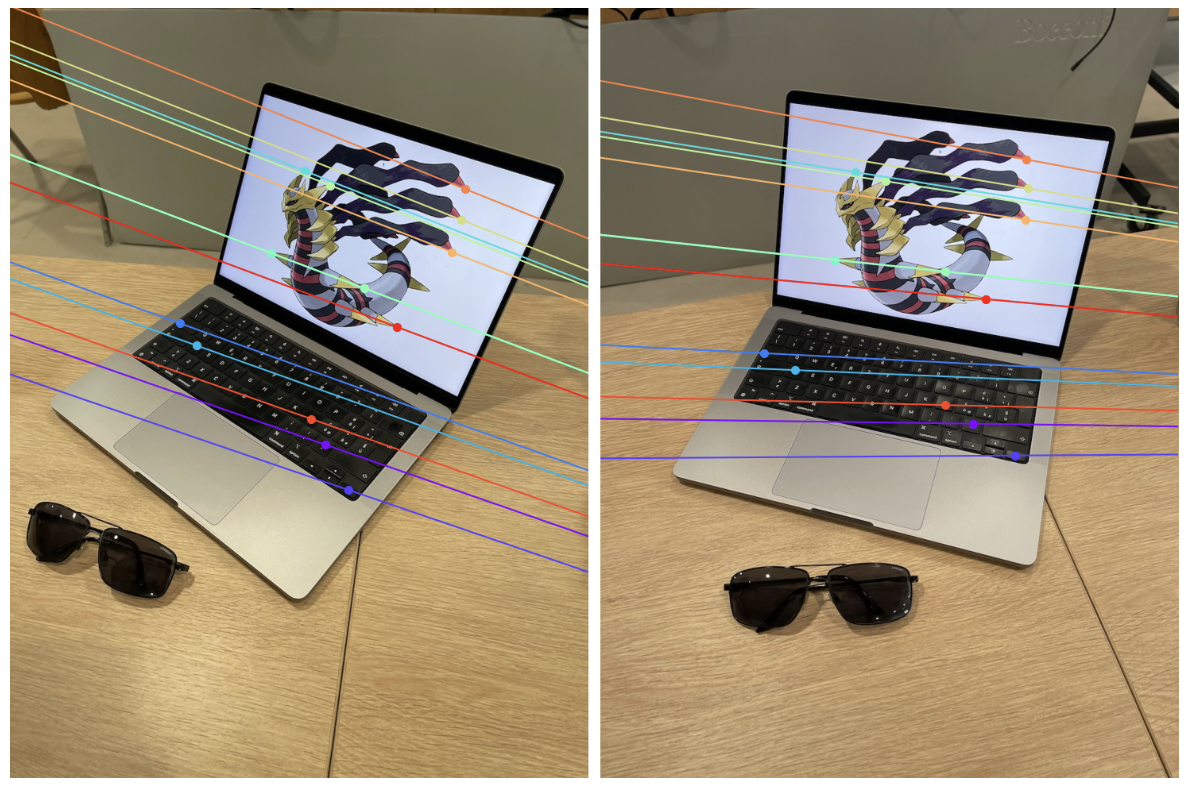
\includegraphics[width=\linewidth]{img/epipolar.png}
        \caption{Epipolar lines for the two views. Each point in one image corresponds to a line in the other image, and all these lines should intersect at the epipole (which is oftentimes outside the visible image).}
        \label{epipolar}
    \end{minipage}
    \hfill
    \begin{minipage}[t]{0.48\textwidth}
        \centering
        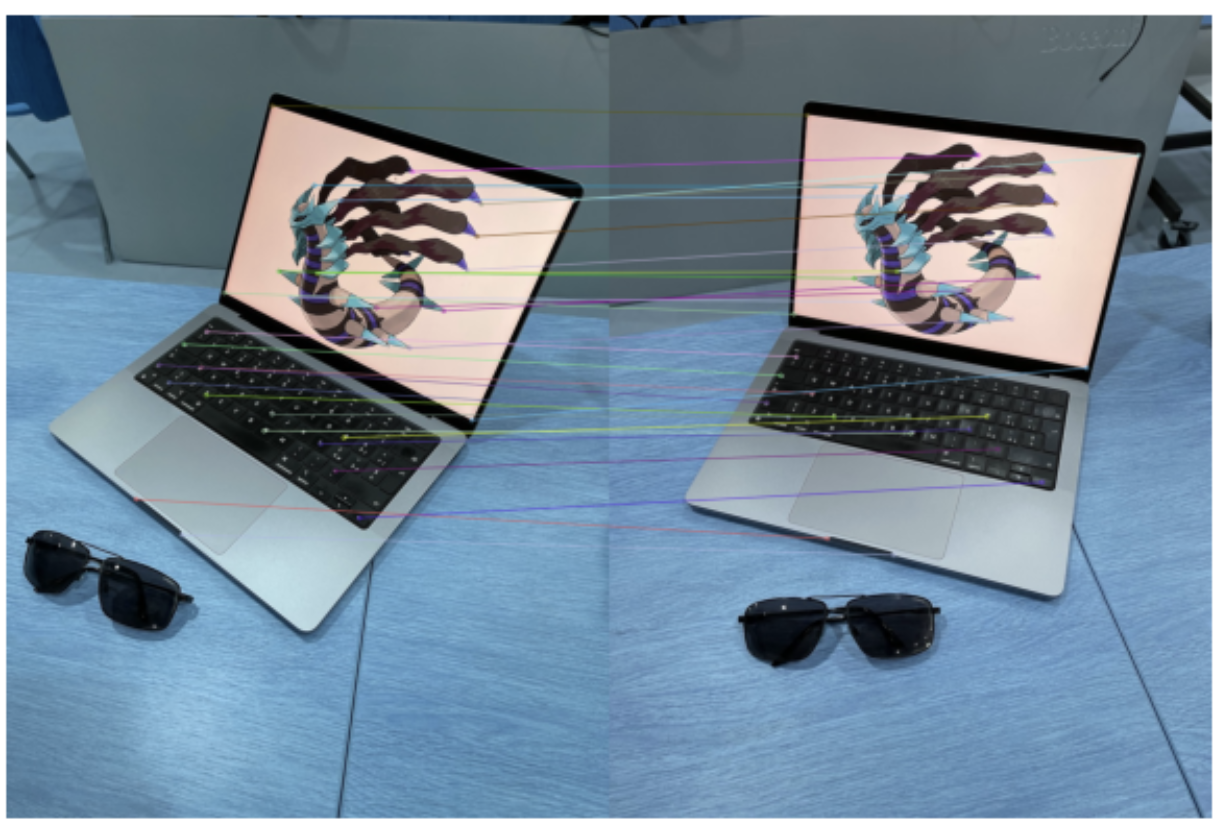
\includegraphics[width=\linewidth]{img/matches.png}
        \caption{Point correspondences between the two images. The lines connect matching points across the two views.}
        \label{matches}
    \end{minipage}
\end{figure}

\paragraph{Results} We test our implementation on a pair of images taken from slightly different viewpoints (Figure \ref{matches}). Using \textit{RANSAC} with $N = 1000$ and $\epsilon = 0.2$, we achieved a mean geometric error of $0.058$ pixels (averaged over all points and over $100$ trials, with a standard deviation of $0.019$ and a max error $0.140$). The algorithm successfully identified $14$ inliers out of the $30$ annotated correspondences, resulting in an inlier ratio of $0.47$.

\paragraph{Discussion} Our implementation of the eight-point algorithm with normalization and RANSAC proved effective in estimating the fundamental matrix and visualizing the epipolar geometry. We observed that normalization significantly improved the numerical stability of the algorithm, while RANSAC successfully handled outliers in the point correspondences.